\documentclass[aps, prd, twocolumn, superscriptaddress, floatfix, showpacs, nofootinbib, longbibliography]{revtex4-1}

% Fixes Adbobe error (131)
\pdfminorversion=4

% Ams math
\usepackage{amsmath}
\usepackage{amssymb}

% Packages for setting figures
\usepackage[]{graphicx}
\usepackage{subfig}

% Colors
\usepackage{color}

% Bibliography
\usepackage{natbib}

\usepackage{placeins}

\usepackage{multirow}

\usepackage{hhline}

% get hyperlinks
%\usepackage{hyperref}

% Tables
\newcommand{\specialcell}[2][c]{%
  \begin{tabular}[#1]{@{}c@{}}#2\end{tabular}}

\newcommand{\fdot}{\dot{f}}
\newcommand{\F}{{\mathcal{F}}}
\newcommand{\twoFhat}{\widehat{2\F}}
\newcommand{\twoFtilde}{\widetilde{2\F}}
\newcommand{\A}{\boldsymbol{\mathcal{A}}}
\newcommand{\blambda}{\boldsymbol{\mathbf{\lambda}}}
\newcommand{\blambdaSignal}{\boldsymbol{\mathbf{\lambda}}^{\rm s}}
\newcommand{\tglitch}{t_{\rm glitch}}
\newcommand{\tstart}{t_{\rm start}}
\newcommand{\tend}{t_{\rm end}}
\newcommand{\Nglitches}{N_{\rm g}}
\newcommand{\Tspan}{T}
\newcommand{\Tcoh}{T_{\rm coh}}
\newcommand{\tref}{t_{\rm ref}}
\newcommand{\Nseg}{N_{\rm seg}}
\newcommand{\Nsteps}{N_{\rm steps}}
\newcommand{\Ntemps}{N_{\rm temps}}
\newcommand{\Nstages}{N_{\rm stages}}
\newcommand{\Nspindown}{N_{\rm spindowns}}
\renewcommand{\H}{\mathcal{H}}
\newcommand{\Hs}{\H_{\rm s}}
\newcommand{\Hn}{\H_{\rm n}}
\newcommand{\ho}{h_0}
\newcommand{\homax}{\ho^{\rm max}}
\newcommand{\Bsn}{B_{\rm S/N}}
\newcommand{\AmplitudePrior}{\Pi_\mathcal{A}}
\newcommand{\mutilde}{\tilde{\mu}}
\newcommand{\Sn}{S_{\rm n}}
\newcommand{\V}{\mathcal{V}}
\newcommand{\Vsky}{\V_{\rm Sky}}
\newcommand{\Vpe}{\V_{\rm PE}}
\newcommand{\smax}{s_{\textrm{max}}}
\newcommand{\fmax}{f_{\textrm{max}}}



% For editing purposes: remove before submition
\usepackage[normalem]{ulem}	%% only added for 'strikeout' \sout
\usepackage[usenames,dvipsnames]{xcolor}

\newcommand{\dcc}{LIGO-{\color{red}}}

%% ---------- editing/commenting macros: make sure all a cleared at the end! ----------
\newcommand{\mygreen}{\color{green!50!black}}
\newcommand{\addtext}[1]{\textcolor{green!50!black}{#1}}
\newcommand{\meta}[1]{\addtext{#1}}
\newcommand{\CHECK}[1]{\textcolor{red}{#1}}
\newcommand{\strike}[1]{\textcolor{red}{\sout{#1}}}
\newcommand{\comment}[1]{\textcolor{red}{[#1]}}
\newcommand{\replace}[2]{\strike{#1}\addtext{$\rightarrow$ #2}}
%% ---------- end: editing/commenting macros ----------------------------------------

\begin{document}

\title{MCMC follow-up methods for continuous gravitational wave candidates}

    \author{G. Ashton}
    \email[E-mail: ]{gregory.ashton@ligo.org}
    \affiliation{Max Planck Institut f{\"u}r Gravitationsphysik
                 (Albert Einstein Institut) and Leibniz Universit\"at Hannover,
                 30161 Hannover, Germany}
    \author{R. Prix}
    \affiliation{Max Planck Institut f{\"u}r Gravitationsphysik
                 (Albert Einstein Institut) and Leibniz Universit\"at Hannover,
                 30161 Hannover, Germany}

\date{\today}

\begin{abstract}
We detail methods to follow-up potential CW signals (as identified by
wide-parameter space semi-coherent searches) leverging MCMC optimisation of the
$\mathcal{F}$-statistic. First, we demonstrate the advantages of such an
optimisation whilst increasing the coherence time, namely the ability to
efficiently sample an evolving distrubution and consider multiple modes.
Subsequently, we illustrate estimation of parameters and the Bayes factor which
can be used to understand the signficance of the candidate. Finally, we explain
how the methods can be simply generalised to allow the waveform model to be
transient or undergo glitches.

\end{abstract}

\pacs{04.80.Nn, 97.60.Jd, 04.30.Db}
\input{git_tag.tex}
\date{\commitDATE; \commitIDshort-\commitSTATUS, \dcc}

\maketitle


\section{Introduction}

A possible target for the advanced gravitational wave detector network of LIGO
and Virgo are long-lived periodic sources called continuous waves (CWs).
Rapidly rotating nonaxisymmetric neutron stars are potentially capable of
producing detectable CWs which last much longer than typical observation spans.
There exists three well known sources of the nonaxisymmetry: `mountains',
precession, and r-mode oscillations; each of which make a prediction for the
scaling between $\nu$, the NS spin frequency and $f$, the gravitational wave
frequency. In any case, observing neutron stars through their gravitational
wave emmission would provide a unique astrophysical insight and has hence
motivated numerous searches.

As shown by \citet{jks1998}, the gravitational wave signal from a
nonaxisymmetric source produces a strain in the detector $h(t, \A, \blambda)$;
where $\A{=}\{h_0, \cos\iota, \psi, \phi_0\}$ is a vector of the four
\emph{amplitude-parameters} (expressed in `physical coordinates') and
$\blambda$ is a vector of the \emph{Doppler-parameters} consisting of the
sky-location, frequency $f$, and any spindown terms required by the search.

CW searches typically use a fully-coherent matched-filtering methods whereby a
template (the signal model at some specific set of parameters) is convolved
against the data resulting in a detection statistic. Since the signal
parameters are unknown, it is usual to perform this matched filtering over a
grid of points.  Three search categories can be identified: \emph{targeted}
searches for a signal from a known electromagnetic pulsar where the Doppler
parameters are considered `known'; \emph{directed} searches in which the
location is known, but not the frequency and spin-down (i.e.  searching for the
neutron star in a supernova remnant which does not have a known pulsar); and
\emph{all-sky} searches where none of the parameters are considered known.
Searching over more parameters amounts to an increase in the dimension of the
search space. Since the density of grid points required to resolve a signal
scales inversely with total coherence time $\Tcoh$ (the span of data used in
a fully-coherent matched filter), wide-parameter searches (such as the all-sky)
with many search dimensions over long durations of data are computationally
demanding.

At a fixed computing cost, it has been shown (see for example \citep{brady1998,
prix2012}) that a semi-coherent search is more sensitive for unknown signals
than a fully-coherent search. While the exact details of how the search works
depends on the implementation, semi-coherent search work by splitting the total
observation span $\Tspan$ into $\Nseg$ segments (each lasting for $\Tcoh$) and
in each segment computes the fully-coherent detection statistic; the
semi-coherent detection statistic is then computed by some combination of all
segments summed at the same point in parameter space. Fundamentally, this gain
in sensitivity is because the width of a peak in the detection statistic due to
a signal is inversely propotional to the cohrence time: shorter coherence times
make the peak wider and hence the a lower density of templates. This idea was
first proposed by \citet{brady2000} along with the first implementation, the
`Stack-slide' search. Since then, several modifications such as the
`Hough-transform' \citep{krishnan2004, astone2014}, and the `Powerflux' method
(first described in \citet{allyskyS42008}) have been proposed, implemented and
applied to gravitational wave searches.

Wide parameter space searches produce a list of candidates with an associated
detection statistic which passes some threshold. In order to verify these
candidates, they are subjected to a \emph{followed-up}: a process of increasing
the coherence time, eventually aiming to calculate a fully-coherent detection
statistic over the maximal span of data. In essense, the semi-coherent search
is powerful as it spreads the significance of a candidate over a wider area of
parameter space, so a follow-up attempts to reverse this process and recover
the maximum significance and tightly constrain the candidate parameters. The
original hierarchical follow-up of \citet{brady2000} proposed a two-stage method
(an initial semi-coherent  stage followed directly by a fully-soherent search.
However, it was shown in a numerical study by \citet{cutler2005} that allowing
an arbitrary number of semi-coherent stages before the final fully-coherent
stage can significantly improve the efficiency: ultimately they concluded that
three semi-coherent stages provide the best trade-off between sensitivity and
computational cost.

The first implementation of a two-stage follow-up was given by
\citet{shaltev2013} and used the Mesh Adaptive Direct Search algorithm for
optimisation. At the time of publication, this method was limited to two stages
and could not handle binary parameters \comment{(I think these limitations have
now been removed, but I can't find a publication)}, however these are practical
limitations which can \comment{(have?)} be overcome.
\comment{Add something on multiple modes?}

In this paper, we propose an alternative hierarchical follow-up procudure using
Markov-Chain Monte-Carlo (MCMCM) as the optimisation tool. In terms of the
semi-coherent to follow-up procedure, an MCMC tool is advantages due to it's
ability to trace the evolution multiple modes simultaneuosly through the
follow-up procudedure and allow the optimisation to decide between them without
arbitrary cuts. In addition, MCMC methods also provide two further
advatanges: they can calculate directly calculate Bayes factors, the significance
of a candidate and because they are `gridless' one can arbitrarily vary the
waveform model without requring an understanding of the underlying topology.
We will exploit this latter property to propose an additional step in the
follow-up procudure which allows for the CW signal to be either a transient-CW
(a periodic signal lasting $\mathcal{O}(\textrm{hours-weeks})$) or to undergo
glitches (as seen in pulsars).

We begin in Section~\ref{sec_hypothesis_testing} with a review of search
methods from a Bayesian perspective. Then in
Section~\ref{sec_MCMC_and_the_F_statistic} we introduce the MCMC optimisation
producedure and give details of our particular implementation. In
Section~\ref{sec_follow_up} we will illustrate applications of the method and
provide a prescription for choosing the setup. In Sections~\ref{sec_transients}
and \ref{sec_glitches} we demonstrate how searches can be performed for either
transient or glitches CWs before we finally conclude in
Section~\ref{sec_conclusion}.

\section{Hypothesis testing}
\label{sec_hypothesis_testing}

\subsection{Bayes factors}
Given some data $x$ and a set of background assumptions $I$, we formulate
two hypotheses: $\Hn$, the data contains solely Gaussian noise and $\Hs$, the
data contains an additive mixture of noise and a signal $h(t; \A, \blambda)$.
In order to make a quantitative comparison, we use Bayes theorum in the usual
way to write the odds as
\begin{equation}
O_{\rm S/N} \equiv \frac{P(\Hs| x, I)}{P(\Hn| x, I)} =
\Bsn(x| I) \frac{P(\Hs| I)}{P(\Hn | I)},
\end{equation}
where the second factor is the prior odds while the first factor is the
\emph{Bayes factor}:
\begin{equation}
\Bsn(x| I) = \frac{P(x| \Hs, I)}{P(x| \Hn, I)}.
\end{equation}
Typically, we set the prior odds to unity such that it is the Bayes factor
which determines our confidence in the signal hypothesis. In this work we will
therefore discuss the Bayes factor with the implied assumption this is
equivalent to the odds, unless we have a good reason to change the prior odds.

We can rewrite the Bayes factor in terms of the two sets of signal parameters
as
\begin{equation}
\Bsn(x| I) = \frac{P(x, \A, \blambda|\Hs, I)}
{P(\A| \Hs, I)P(\blambda| \Hs, I)P(x| \Hn, I)}.
\end{equation}
Marginalising over the two sets of parameters we find that
\begin{equation}
\Bsn(x| I)= \iint
\mathcal{L}(x; \A, \blambda)
P(\A| \Hs, I)P(\blambda| \Hs, I)
d\blambda d\A
\label{eqn_full_bayes}
\end{equation}
where
\begin{equation}
\mathcal{L}(x; \A, \blambda) \equiv \frac{P(x |\A, \blambda, \Hs, I)}{P(x| \Hn, I)},
\label{eqn_likelihood}
\end{equation}
is the \emph{likelihood-ratio}.

At this point, we can appreciate the problems of searching for unknown signals:
one has four amplitude parameters and several doppler parameters (three plus
the number of spin-down and binary parameters) over which this integral must be
performed. If a single signal exists in the data, this corresponds to a single
peak in the likelihood-ratio, but at an unknown location. Therefore, one must
must first search for peaks (candidates), and then subsequently analyse their
significance. If one has prior knowledge this can be used; for example in
targeted searches for gravitational waves from known pulsars emitting CWs from
a mountain the Doppler parameters are considered known collapsing their
integral to a single evaluation.

\subsection{The $\F$-statistic}

For directed and all-sky searches, a common method introduced by
\citet{jks1998} to reduce the parameter space is the maximum-likelihood
approach. In this approach (often referred to as `frequentist'), one starts by
defining the likelihood-ratio, Equation~\eqref{eqn_likelihood}, which in this
context is a \emph{matched-filtering} amplitude. Then, analytically maximising
this likelihood-ratio with respect to the four amplitude parameters results
(c.f.~\citet{prix2009}) in a maximised log-likelihood given by $\F(x|
\blambda)$: the so-called $\F$-statistic. Picking a particular set of Doppler
parameters $\blambda$ (the template) one can then compute a detection statistic
(typicaly $2\F$ is used) which can be used to quantify the significance of the
template. Usually this is done by calculating a corresponding false alarm rate,
the probability of seeing such a detection statistic in Gaussian noise.

Calculations of the significance are possible due to the properties of the
detection statistic: in Gaussian noise, it can be shown \citep{jks1998,
cutlershutz2005} that $\widetilde{2\F}$ follows a chi-squared distribution with
4 degrees of freedom. In the presence of a signal, $\widetilde{2\F}$ is
still chi-squared with 4 degrees of freedom, but has a non-centrality parameter
$\tilde{\rho}^{2}$ such that its expectation value is
\begin{equation}
\textrm{E}[\widetilde{2\F}(x; \blambda)] = 4 + \tilde{\rho}(x; \blambda)^2.
\label{eqn_twoF_expectation}
\end{equation}
The non-centrality parameter in this context is the SNR of the matched-filter
given by
\begin{equation}
\rho^{2} = (h | h) \propto \frac{h_0^2}{\Sn}\Tcoh \mathcal{N}
\end{equation}
where $(h|h)$ is the inner product of the signal with itself (see for example
\citet{prix2009}), $\Sn$ is a (frequency-dependent) measure of the noise in
the detector and $\mathcal{N}$ is the number of detectors.


\subsection{Using the $\F$-statistic to compute a Bayes factor} At first, it
appears that the $\F$-statistic is independent of the Bayesian framework since
it was first derived directly from the likelihood. However, it was shown by
\citet{prix2009} that if we marginalise over the four amplitude parameters of
Equation~\eqref{eqn_full_bayes}, choosing a prior $\Pic$ such that
\begin{equation}
P(\A| \Hs, \Pic, I) \equiv \left\{
\begin{array}{ll}
C & \textrm{ for } \ho < \homax \\
0 & \textrm{ otherwise}
\end{array}
\right..
\end{equation}
then the integral, when $\homax \gg 1$, is a Gaussian integral and can be
computed analytically as
\begin{align}
\Bsn(x| \Pic, \blambda, I) & \equiv
\int
\mathcal{L}(x ;\A, \blambda)
P(\A| \Hs, I) d\A
\\
& = \frac{C (2\pi)^{2} e^{\F(x| \blambda)}}
{\sqrt{\textrm{det} \mathcal{M}}},
\end{align}
where $C$ is a normalisation constant, $\textrm{det}\mathcal{M}$ is an antenna
pattern factor dependent on the sky-position and observation period, and
$\mathcal{F}$ is the frequentist log-likelihood of \citet{jks1998}. This result
demonstrates that the $\mathcal{F}$-statistic is proportional to the log-Bayes
factors when calculated with a uniform prior on the amplitude parameters and
fixed Doppler parameters.

As such, we can define the Bayes-factor of Equation~\eqref{eqn_full_bayes} as
\begin{equation}
\Bsn(x| \Pic, I) = \int
\Bsn(x| \Pic, \blambda, I) P(\blambda| \Hs, I)
 d\blambda,
\end{equation}
or neglecting the constants
\begin{equation}
\Bsn(x| \Pic, I) \propto \int
e^{\F(x| \blambda)} P(\blambda| \Hs, I)
 d\blambda.
\label{eqn_bayes_over_F}
\end{equation}

Formulating the significance of a CW candidate in this way is pragmatic in that
there exists a wealth of well-tested tools \citep{lalsuite} capable of
computing the $\mathcal{F}$-statistic for CW signals, transient-CWs, and CW
signals from binary systems; these can be levereged to compute
Equation~\eqref{eqn_bayes_over_F}, or adding in the constant
$\Bsn(x| \Pic)$ itself. The disadvantage to this method is that
we are forced to use the prior $\Pic$, which was shown by \citet{prix2009} to
be unphysical.

\section{MCMC and the $\mathcal{F}$-statistic}
\label{sec_MCMC_and_the_F_statistic}

The MCMC class of optimisation tools are formulated to solve the problem of
infering the posterior distribution of some general model parameters $\theta$
given given some data $x$ for some hypothesis $\H$. Namely, Bayes rule
\begin{equation}
P(\theta| x, \H, I) \propto P(x| \theta, \H, I)P(\theta| \H, I),
\label{eqn_bayes_for_theta}
\end{equation}
is used to evaluate proposed jumps from one point in parameter to other points;
jumps which increase this probabily are accepted with some probability. The
algorithm, proceeding in this way, is highly efficient at resolving peaks in
high-dimension parameter spaces.

At this point, we note the equivalence of Equation~\eqref{eqn_bayes_for_theta}
to the integrand of Equation~\eqref{eqn_bayes_over_F}:
\begin{equation}
P(\blambda | x, \Pic, \Hs, I)
%=\Bsn(x| \Pic, \blambda) P(\blambda| \Hs I).
\propto e^{\F(x| \blambda)} P(\blambda| \Hs I),
\label{eqn_lambda_posterior}
\end{equation}
where $e^{\F}$ is the likelihood.
In this work, we will focus on using MCMC methods to sample this, the
posterior distribution of the Doppler parameters and moreover compute the
final Bayes factor.

\subsection{The \texttt{emcee} sampler}

In this work we will use the \texttt{emcee} ensemble sampler
\citep{foreman-mackay2013}, an implementation of the affine-invariant ensemble
sampler proposed by \citet{goodman2010}. This choice addresses a key issue with
the use of MCMC sampler, namely the choice of \emph{proposal distribution}. At
each step of the MCMC algorithm, the sampler generates from some distribution
(known as the proposal-distribution) a jump in parameter space. Usualy, this
proposal distribution must be `tuned' so that the MCMC sampler effeciently
walks the parameter space without either jumping too far off the peak, or
taking such small steps that it takes a long period of time to traverse the
peak. The \texttt{emcee} sampler addresses this by using an ensemble, a large
number ${\sim}100$ parallel \emph{walkers}, in which the proposal for each
walker is generated from the current distribution of the other walkers.
Moreover, by applying an an affine transformation, the efficiency of the
algorithm is not diminished when the parameter space is highly anisotropic. As
such, this sampler requires little in the way of tuning: a single proposal
scale and the number of steps to take.

\subsection{Parallel tempering: sampling multimodal posteriors}
Beyond the standard ensemble sampler, we will also use one further
modification, the parallel-tempered ensemble sampler. A parallel
tempered MCMC simulation, first proposed by \citet{swendsen1986}, runs
$\Ntemps$ simulations in parallel with the likelihood in the $i^{\rm th}$
parallel simulation is raised to a power of $1/T_{i}$ where $T_i$ is referred
to as the temperature. As such, Equation~\eqref{eqn_lambda_posterior} is
written as
\begin{equation}
P(\blambda | T_i, x, \Pic, \Hs, I)
%=\Bsn(x| \Pic, \blambda)^{T_i} P(\blambda| \Hs I).
\propto (e^{\F(x| \blambda)})^{T_i} P(\blambda| \Hs I).
\end{equation}
Setting $T_0=1$ with $T_i > T_0 \; \forall \; i > 1$, such that the lowest
temperature recovers Equation~\eqref{eqn_lambda_posterior} while for higher
temperatures the likelihood is broadened (for a Gaussian likelihood, the
standard devitation is larger by a factor of $\sqrt{T_i}$). Periodically, the
algorithem swaps the position of the walkers between the different
temperatures. This allows the $T_0$ chain (from which we draw samples of the
posterior) to efficiently sample from multi-modal posteriors. This introduces
two additional tuning parameters, the number and range of the set of
temperatures $\{T_i\}$, we will discuss their signficance when relevant.

\subsection{Parallel tempering: estimating the Bayes factor}
In addition, parallel-tempering also offers a robust method to estimate the
Bayes factor of Equation~\eqref{eqn_bayes_over_F}. If we define
$\beta\equiv1/T$, the inverse temperature and $Z(\beta)\equiv \Bsn(x| \Pi_{\rm
c}, I)$, then as noted by \citet{goggans2004} for the general case, we may
write
\begin{align}
\frac{1}{Z} \frac{\partial Z}{\partial \beta}=
\frac{
\int \Bsn(x| \Pic, \blambda)^{\beta}
\log(\Bsn(x| \Pic, \blambda))P(\blambda| I)
d\blambda
}
{
\int \Bsn(x| \Pic, \blambda)^{\beta})P(\blambda| I)
d\blambda
}
\end{align}
The right-hand-side expresses the average of the log-likelihood at $\beta$. As
such, we have
\begin{align}
\frac{\partial \log Z}{\partial \beta} = 
\langle \log(\Bsn(x| \Pic, \blambda) \rangle_{\beta}
\end{align}
The log-likelihood are a calculated during the MCMC sampling. As such, one
can numerically integrate to get the Bayes factor, i.e.
\begin{align}
\log \Bsn(x| \Pic, I) = \log Z = \int_{0}^{1}
\langle \log(\Bsn(x| \Pic, \blambda) \rangle_{\beta} d\beta.
\end{align}
In practise, we use a simple numerical quadrature over a finite ladder of
$\beta_i$ with the smallest chosen such that choosing a smaller value does not
change the result beyond other numerical uncertainties. Typically, getting
accurate results for the Bayes factor requires a substantially larger number of
temperatures than are required for effeciently sampling multi-modal
distributions.  Therefore, it is recomended that one uses a small number of
temperatures during the search stage, and subsequently a larger number of
temperatures (suitably initialised close to the target peak) when estimating
the Bayes factor.

\subsection{The topology of the likelihood}

We intend to use the $\F$-statistic as our log-likelihood in MCMC simulations,
but before continuing, it is worthwhile to acquaint ourselves with the typical
behaviour of the log-likelihood by considering a specific example.

As shownn in Equation~\eqref{eqn_twoF_expectation}, the expectation of
$\widetilde{2\F}$ is 4 in Gaussian noise alone, but proportional to the square
of the SNR in the presense of a signal.  To illustrate this, let us consider
$\widetilde{2\F}$ as a function of $f$ (the template frequency) if there exists
a signal in the data with frequency $f_0$. We will assume that all other
Doppler parameters are perfectly matched.  Such an example can be calculated
analytically, taking the matched-filtering amplitude (Equation~(11) of
\citep{prix2005}) with $\Delta\Phi(t) = 2\pi(f - f_0) t$, the expectation of
$\widetilde{2\F}$ as a function of the template frequency $f$ is given by
\begin{equation}
\textrm{E}[\widetilde{2\F}](f) = 4 + 
(\textrm{E}[\widetilde{2\F_0}] -4)\textrm{sinc}^{2}(\pi(f-f_0)\Tcoh))
\label{eqn_grid_prediction}
\end{equation}
where $\textrm{E}[\widetilde{2\F_0}]$ is the expected $\widetilde{2\F}$ for
a perfectly matched signal (when $f=f_0$).

In Figure~\ref{fig_grid_frequency} we compare the analytic prediction of
Equation~\eqref{eqn_grid_prediction} with the value computed numerically
from simulating a signal in Gaussian noise. As expected, close to the signal
frequency $f_0$ the detection statistic peaks with a a few local secondary
maxima. Away from this frequency, in Gaussian noise, we see many local maxima
centered around the expected value of 4.
\begin{figure}[htb]
\centering 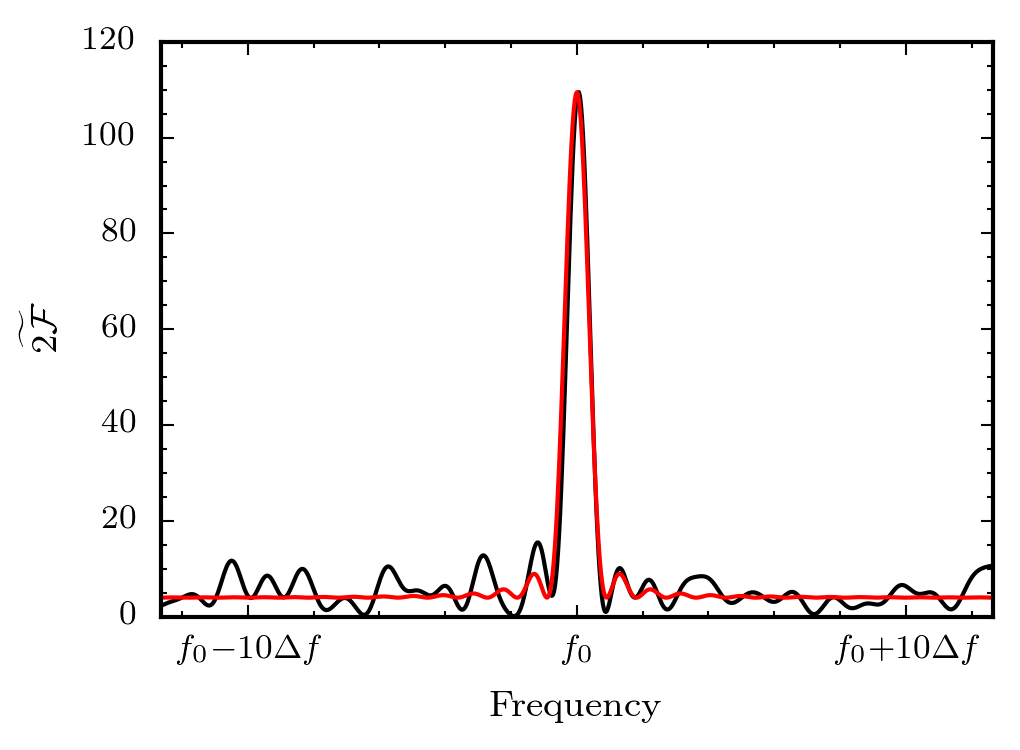
\includegraphics[width=0.45\textwidth]{grided_frequency_search_1D}
\caption{Comparison of the analytic prediction of
Equation~\eqref{eqn_grid_prediction} (in red) with the value computed
numerically from simulating a signal in Gaussian noise (in black).
\comment{Need to explain ticks}}
\label{fig_grid_frequency}
\end{figure}

\subsection{Limitations of use}

In general, MCMC samplers are highly effective in generating samples of the
posterior in multi-dimensional parameter spaces. However, they will perform
poorly if the posterior has multiple small maxima with only a small number of
large maxima which occupy a small fraction of the prior volume. Since we will
use $\F$ as our log-likelihood, Figure~\ref{fig_grid_frequency} provides an
example of the space we will ask the sampler to explore. Clearly, if the width
of the signal peak is small compared to the prior volume, the sampler will get
`stuck' on the local maxima and be ineffecient at finding the global maxima.
This problem is excabated in higher-dimensional search spaces where the volume
fraction of the signal scales with the exponent of the number of dimensions.

In a traditional CW search which uses a grid of templates (also known as a
template bank), the spacings of the grid are chosen such that the loss of
signal to noise ratio (SNR) is bounded to less than $u$, the template-bank
mismatch. The optimal choice of grid then consists of minimising the computing
cost while respecting this minimum template-bank mismatch or vice-verse (for
examples see \citet{pletsch2010, prix2012, wette2013, wette2015}). We will now
discuss how the work on setting up these grids can be applied to the problem of
determining whether the setup is appropriate for an MCMC method: i.e. given the
prior volume do we expect a signal to occupy a non-negligible volume?

For a fully-coherent $\F$-statistic search on data containing Gaussian noise
and a signal with Doppler parameters $\blambdaSignal$, the template-bank
mismatch at the grid point $\blambda_{l}$ is defined to be
\begin{align}
\mutilde(\blambdaSignal, \blambda_{l}) \equiv 1 - 
\frac{\tilde{\rho}(\blambda_l;\blambdaSignal)^{2}}
{\tilde{\rho}(\blambdaSignal; \blambdaSignal)^{2}},
\end{align}
where $\tilde{\rho}(\blambda_l; \blambdaSignal)$ is the non-centrality
parameter (c.f. Equation~\ref{eqn_twoF_expectation}) at $\blambda_l$, given
that the signal is at $\blambdaSignal$. As such
$\widetilde{\textrm{SNR}}(\blambdaSignal; \blambdaSignal)$ is the
perfectly-matched non-centrality parameter, for which the mismatch is zero.
For a fully-coherent search, this non-centrality parameter is equivalent to
fully-coherent matched-filter signal to noise ratio SNR. However,
as noted by \citet{leaci2015}, this is true for the fully-coherent case only.
Therefore, we will use the non-centrality parameter which easily generalised to
the semi-coherent case.

To make analytic calculations of the mismatch possible, as first shown by
\citet{brady1998}, the mismatch can be approximated by
\begin{equation}
\mutilde(\blambda, \Delta\blambda) \approx 
\tilde{g}_{\alpha \beta}^{\phi} \Delta\lambda^{\alpha}\Delta\lambda^{\beta}
+ \mathcal{O}\left(\Delta\blambda^{3}\right)
\end{equation}
where we switch to using index notation for which we sum over repeated indices.
Here, $\tilde{g}_{\alpha\beta}^{\phi}$ is the `phase-metric' given by
\begin{align}
\tilde{g}^{\phi}_{\alpha \beta}(\blambda) = 
\langle 
\partial_{\Delta\lambda^{\alpha}}\phi
\partial_{\Delta\lambda^{\beta}}\phi
\rangle
-
\langle 
\partial_{\Delta\lambda^{\alpha}}\phi
\rangle
\langle
\partial_{\Delta\lambda^{\beta}}\phi
\rangle,
\label{eqn_metric}
\end{align}
where $\langle \cdot \rangle$ denotes the time-average over $\Tcoh$ and
$\phi(t; \blambda)$ is the phase evolution of the source. The phase metric is
in fact an approximation of the full metric which includes modulations of the
amplitude parameters $\A$; it was shown by \citet{prix2007metric} that it is a
good approximation when using data spans longer than a day and data from
multiple detectors. 

The phase metric, Equation~\eqref{eqn_metric} provides the neccesery tool to
measure distances in the Doppler parameter space in units of mismatch. To
calculate it's components, we define the phase evolution
of the source as \citep{wette2015}
\begin{align}
\phi(t; \blambda) \approx 2\pi\left(
\sum_{s=0}^{\smax} f^{(s)}\frac{(t-\tref)^{s+1}}{(s+1)!}
+ \frac{r(t)\cdot\mathbf{n}}{c} \fmax\right),
\label{eqn_phi}
\end{align}
where $\mathbf{n}(\alpha, \delta)$ is the fixed position of the source with
respect to the solar system barycenter (with coordinates $\alpha, \delta$ the
right ascension and declination), $f^(s)\equiv d^{s}\phi/dt^s$, and $\fmax$
a constant chosen conservatively to be the maximum frequency over the data
span.

The frequency and spin-down components of the metric can be easily calculated
due to their linearity in Equation~\eqref{eqn_phi} and for the special case in
which $\tref$ is in the middle of the data span, the frequency and spin-down
parts of the metric are diagonal. Accurately approximating the sky components
of the metric is non-trivial, but was accomplished by \citet{wette2013} for the
fully-coherent case. In \citet{wette2015} it was shown how the calculate the
equivalent semi-coherent metric $\hat{g}_{\alpha\beta}^{\phi}(\blambda,
\Nseg)$.  In the following, we will work with this calculation with the
understanding that $\hat{g}_{\alpha\beta}^{\phi}(\blambda, \Nseg{=}1)=
\tilde{g}_{\alpha\beta}^{\phi}(\blambda)$.

To understand the volume of parameter space which a true signal would occupy,
we can make use of the \emph{metric-volume} \citep{prix2007}, given by
\begin{align}
\mathcal{V} = \int 
\sqrt{\textrm{det}\hat{g}^{\phi}_{\alpha\beta}(\blambda, \Nseg)} d\blambda \approx 
\sqrt{\textrm{det}\hat{g}^{\phi}_{\alpha\beta}(\blambda, \Nseg)} \Delta\blambda
\end{align}
where in the second step we assume a constant coefficient metric. Here, $\Delta
\blambda$ is the volume element which is given by 
\begin{equation}
\Delta\lambda = \frac{\Delta\Omega}{2}
%\frac{1}{2}\sin\delta\Delta\delta\Delta\alpha
\prod_{s=0}^{\smax} \Delta f^{(s)},
\end{equation}
where $\Delta\Omega$ is the solid angle of the sky-patch which is searched,
$\Delta f^(s)$ is the extend of the frequency and spin-down range(s) searched,
and the factor of $1/2$ comes from converting the normalised determinant which
is computed over the whole sky to the solid angle of the directed search.
\comment{Not sure I fully understand this yet, or have really derived it properly}.

The metric volume $\V$ is the approximate number of templates required to cover
the the given Doppler parameter volume at a fixed mismatch of $\approx 1$. As
such, its inverse gives the approximate (order of magnitude) volume fraction of
the search volume which would be occupied by a signal. This can therefore be
used as a proxy for determing if an MCMC search will operate in a regime where
it is effecicient (i.e. where the a signal occupes a reasonable fraction of the
search volume).

The volume $\V$ combines the search volume from all search dimensions. However,
let us know discuss how we can delve deeper to understand how each dimension
contributes to the total product. This is done by noticing that the metric has
a particular block form:
\begin{align}
g_{ij} = \left[
\begin{array}{cc}
g^{\rm Sky} & 0 \\
0 & g^{\rm PE}
\end{array}
\right]
\end{align}
where $g^{\rm Sky}$ is the $2\times2$ sky-metric, while $g^{\rm PE}$ is the
$(\smax{+}1){\times}(\smax{+}1)$ phase-evolution metric.
As such, the volume can be decomposed as
\begin{align}
\mathcal{V} & =
\sqrt{\textrm{det}g^{\rm Sky}}\frac{\Delta\Omega}{2} \times
\sqrt{\textrm{det}g^{\rm PE}}\prod_{s=0}^{\smax}\Delta f^{(s)} \\
& = \Vsky \times \Vpe.
\label{eqn_metric_volume}
\end{align}
Moreover, if $\tref$ is in the middle of the observation span, the diagonal
nature of $g^{\rm PE}$ means that one can further identify
\begin{align}
\Vpe = \prod_{s=0}^{\smax}\sqrt{g^{\rm PE}_{ss}} \Delta f^{(s)}
= \prod_{s=0}^{\smax}\Vpe^{(s)}
\end{align}
This decomposition may be useful in setting up MCMC searches.

\subsection{Example: signal in noise}

In order to familiarise the reader with the features of an MCMC search, we will
now describe a simple directed search (over $f$ and $\dot{f}$) for a simulated
signal in Gaussian noise. The signal will have a frequency of $30$~Hz and a
spin-down of $-1{\times}10^{-10}$~Hz/s, all other Doppler parameters are
`known' and so are irrelevant. Moreover, the signal has an amplitude
$h_0=10^{-24}$~Hz$^{-1/2}$ while the Gaussian noise has
$\Sn=10^{-23}$~Hz$^{-1/2}$ such that the signal has a depth of 10.

First, we must define a prior for each search parameter Typically, we recomend
either a uniform prior bounding the area of interest, or a normal distribution
centered on the target and with some well defined width. However, to ensure
that the MCMC simulation has a reasonable chance at finding a peak, one should
consider the corresponding metric-volume given in
Equation~\eqref{eqn_metric_volume}. For this example, we will use a uniform
prior with a frequency range of $\Delta f = 10^{-7}$~Hz and a spin-down range
of $\Delta \fdot=10^{-13}$~Hz/s both centered on the simulated signal frequency
and spin-down rate. We set the reference time to coincide with the middle of
the data span, therefore the metric volume can be decomposed into the frequency
contribution and spin-down contribution:
frequency,
\begin{align}
\Vpe^{(0)} = \frac{(\pi\Tcoh\Delta f)^2}{3} \approx 2.46
\end{align}
and
\begin{align}
\Vpe^{(1)} = \frac{4(\pi\Delta \fdot)^2\Tcoh^{4}}{45} \approx 48.9
\end{align}
such that $\V\approx120$ (note that $\Vsky$ does not contribute since we do
not search over the sky parameters). This metric volume indicates that the
signal will occupy about 1\% of the prior volume, therefore the MCMC is
expected to work. Alternative priors will need careful thought about how to
translate them into a metric volume: for example using a Guassian one could use
the standard deviation as a proxy for the allowed search region.

In addition to defining the prior, one must also consider how to
\emph{initialise} the walkers. If the prior genuinely represents the stated
prior knowledge, the usual solution is to initialise the walkers from the
prior: that is the starting position is drawn from the prior. However,
instances do occur when one would like to initialise the walkers from a
different distribution. For example, if one only needs to estimate the evidence
(given a particular prior), but is aware from previous searches that the only
significant peak lies in a small area of parameter space, one could initialise
the walkers in a small cluster close to that area. In this example, we
initialise the walkers from the prior such that they have the chance to explore
the entire prior volume.

Having defined the prior, the final setup step is to define the number of
\emph{burn-in} and \emph{production} steps the sampler should take and the
number of walkers; this is a tuning parameter of the MCMC algorithm. The number
of walkers should be typically a few hundred, the greater the number the more
samples will be taken resulting in improved posterior estimates. The burn-in
steps refers to an initial set of steps which are discarded as they are taken
whilst the walkers converge. After they have convereged the steps are known as
production steps since they are used to produce posterior estimates and
calculate the marginal likelihood.

Using these choices, the simulation is run. To illustrate the full MCMC
process, in Figure~\ref{fig_MCMC_simple_example} we plot the progress of all
the individual walkers (each represented by an individual line) as a function
of the total number of steps. The red portion of steps are burn-in and hence
discarded, from this plot we see why: the walkers are initialised from the
uniform prior and initially spend some time exploring the whole parameter space
before congerging. The fact that they converge to a single unique point is due
to the strength of the signal (substantially elevating the likelihood about
that of Gaussian fluctuations) and the tight prior which was quantifed throug the
metric volume $\V$. The production samples, colored black, are only taken once
the sampler has converged - these can be used to generate posterior plots.
\begin{figure}[htb]
\centering
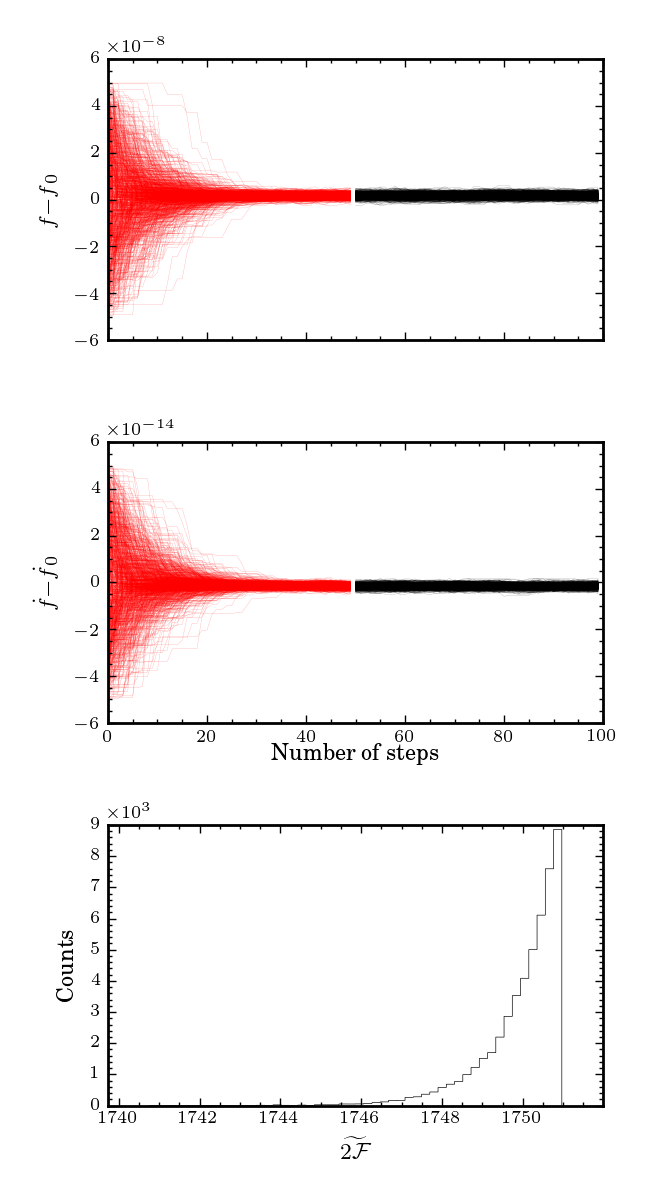
\includegraphics[width=0.5\textwidth]{fully_coherent_search_using_MCMC_walkers}
\caption{The progress of the MCMC simulation for a simulated signal in Gaussian
noise, searching over the frequency and spin-down. The upper two panels show
the position of all walkers as a function of the number of steps for the
frequency and spin-down; when they are colored red the samples are discarded as
burn-in (the first 100 steps), while when they are colored black they are used
as production samples. The bottom panel shows the distribution of
$\widetilde{2\F}$ taken from the production samples.}
\label{fig_MCMC_simple_example}
\end{figure}

\subsection{Example: noise-only}

\section{Follow-up}
\label{sec_follow_up}

Incoherent detection statistics trade significance (the height of the peak) for
sensitivity (the width of the peak). We will now discuss the advantages of
using an MCMC sampler to follow-up a candidate found incoherently, increasing
the coherence time until finally estimating it's parameters and significance
fully-coherently. We begin by rewritting Equation~\eqref{eqn_lambda_posterior},
the posterior distribution of the Doppler parameters, with the explicit
dependence on the coherence time $\Tcoh$:
\begin{equation}
P(\blambda | \Tcoh, x, \Pic, \Hs, I)
%=\Bsn(x| \Tcoh, \Pic, \blambda) P(\blambda| \Hs I).
\propto e^{\hat{\F}(x| \Tcoh, \blambda)} P(\blambda| \Hs I).
\end{equation}

Introducing the coherent time $\Tcoh$ as a variable provides an ability to
adjust the likelihood. Therefore, a natural way to perform a follow-up is to
start the MCMC simulations with a short coherence time (such that the signal
peak occupies a substantial fraction of the prior volume). Subsequently,
incrementally increase this coherence time in a controlled manner, aiming to
allow the MCMC walkers to converge to the new likelihood before again
increasing the coherence time. This can be considered analogous to simulated
annealing (where the likelihood is raised to a power $1/T$ and subseuqntly
`cooled') with the important difference that the semi-coherent likelihood is
wider at short coherence times (rather than flatter as in the case of
high-temperature simulated annealing stages).

To illustrate the utility of this method, in Figure~\ref{fig_follow_up} we show
the progress of the MCMC sampler during such a follow-up. The data, 100 days
from a single detector, consists of Gaussian noise with
$\sqrt{\Sn}=10^{-23}$~Hz$^{-1/2}$ (at the fiducial frequency of the signal) and
a signal. The signal has an amplitude $h_0=1.4\times10^{25}$ such that the
signal has a depth of $\sqrt{\Sn}/h_0=70$ in the noise. The search setup is
outlined in Table~\ref{tab_weak_signal_follow_up}.

\begin{table}[htb]
\caption{The search setup used in Figure~\ref{fig_follow_up}}
\label{tab_weak_signal_follow_up}
\begin{tabular}{c|cccccc}
Stage & $\Nseg$ & $\Tcoh^{\rm days}$ &$\Nsteps$ & $\V$ & $\Vsky$ & $\Vpe$ \\ \hline
0 & 93 & 1.1 & 100 & 10.0 & 1.0 & 10.0 \\
1 & 43 & 2.3 & 100 & $1{\times}10^{2}$ & 6.0 & 20.0 \\
2 & 20 & 5.0 & 100 & $1{\times}10^{3}$ & 30.0 & 50.0 \\
3 & 9 & 11.1 & 100 & $1{\times}10^{4}$ & $1{\times}10^{2}$ & $1{\times}10^{2}$ \\
4 & 4 & 25.0 & 100 & $1{\times}10^{5}$ & $6{\times}10^{2}$ & $2{\times}10^{2}$ \\
5 & 1 & 100.0 & 100,100 & $1{\times}10^{6}$ & $1{\times}10^{3}$ & $9{\times}10^{2}$ \\
\end{tabular}

\end{table}

\begin{figure}[htb]
\centering
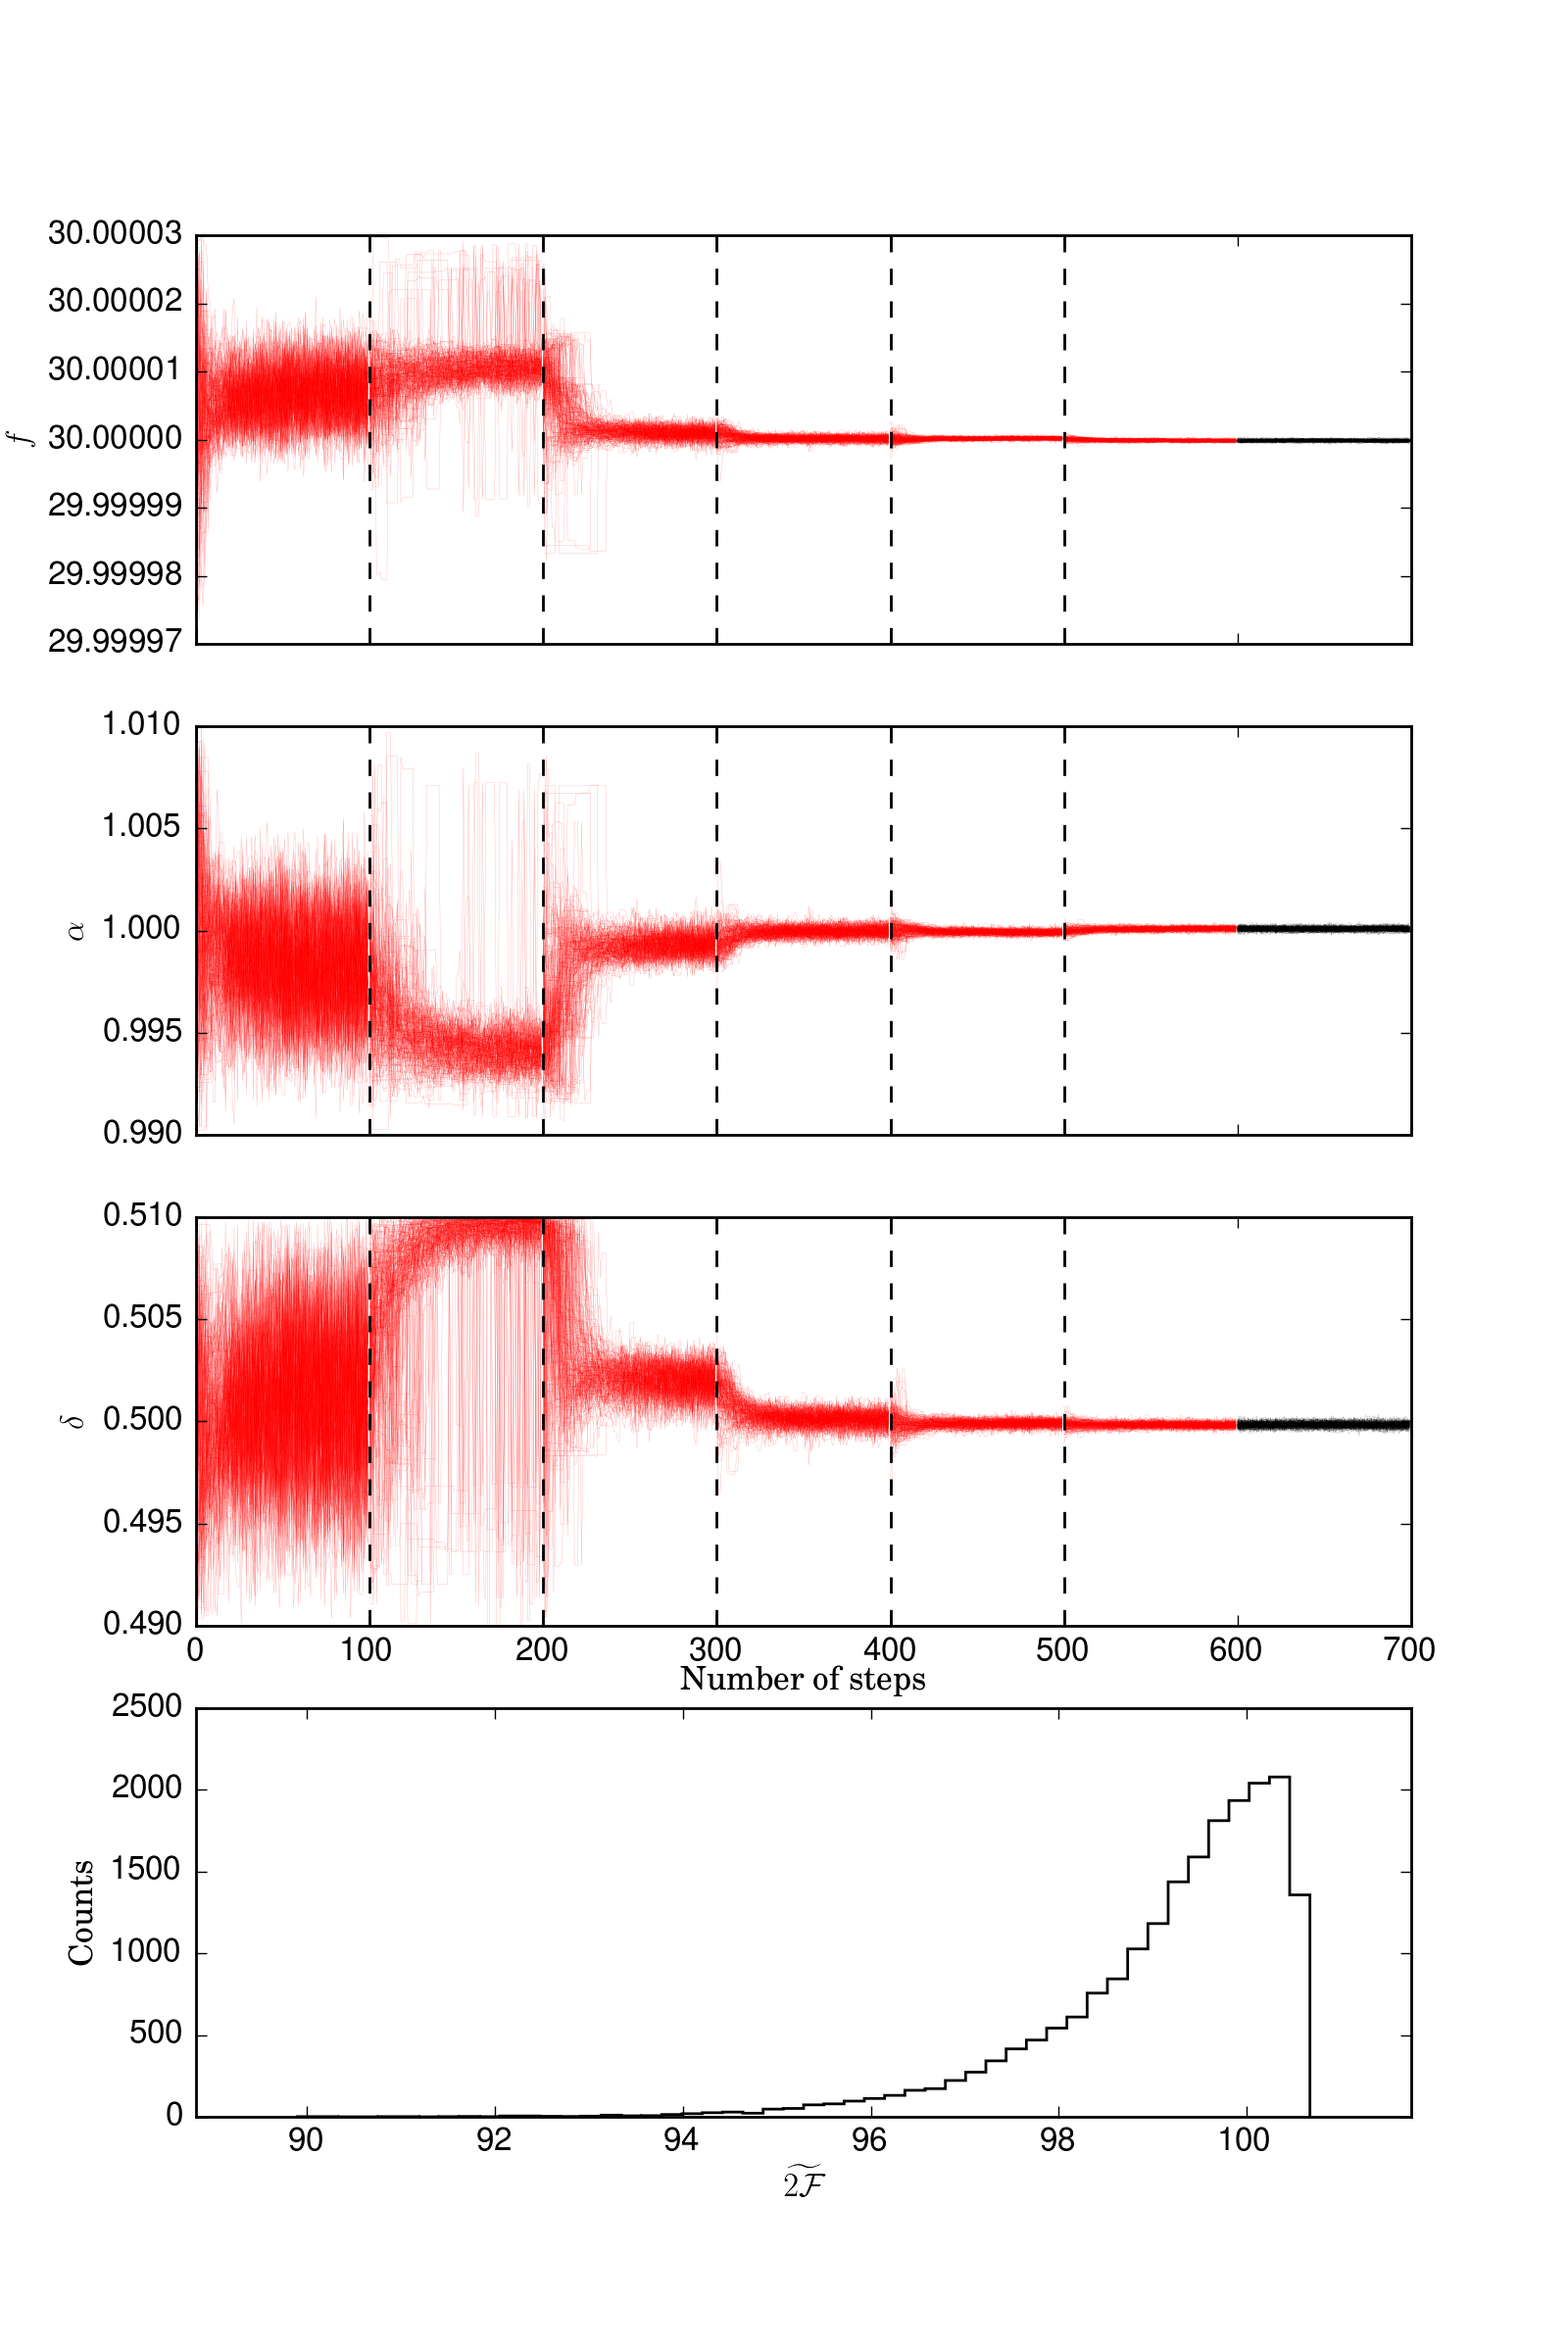
\includegraphics[width=0.5\textwidth]{weak_signal_follow_up_walkers}

\caption{In the top three panels we show the progress of the 500 parallel
walkers (each of which is an individual thin line) during the MCMC simulation
for each of the search parameters, frequency $f$, right-ascension $\alpha$ and
declination $\delta$. Each vertical dashed line indicates the start of a new
stage of the search, the parameters for all stages are listed in
Table~\ref{tab_weak_signal_follow_up}. Samples for use in estimating
posteriors, or other processes are taken from those samples colored black,
which we call the production samples.  The period for which the lines are
coloured red, the samples are discarded either because they are taken from the
posterior when $\Tcoh < \Tspan$, or they are from the burn-in of the final
stage. In the final panel we plot the estimated distribution of
$\widetilde{2\F}$ taken from the production samples.}

\label{fig_follow_up}
\end{figure}

\section{Alternative waveform models: transients}
\label{sec_transients}

\section{Alternative waveform models: glitches}
\label{sec_glitches}

\section{Conclusion}
\label{sec_conclusion}



\section{Acknowledgements}

\bibliography{bibliography}

\end{document}
